\subsection{O2: where the classical estimator fails}
\label{sec:sweep}
Every test source (16 Kodak images, 16 rendered text pages, 24 sharp CCPD plates) is blurred at
8 angles $\times$ 5 lengths $\times$ 4 noise levels. Text and plates are evaluated in a
$96\times256$ window; Kodak images both at full frame ($512\times768$) and cut to the same window,
which separates the effect of \emph{content} from that of \emph{region size}. A trial succeeds
when the angle is within $5^\circ$ and the length within 2\,px.

\begin{figure}[h]
\centering
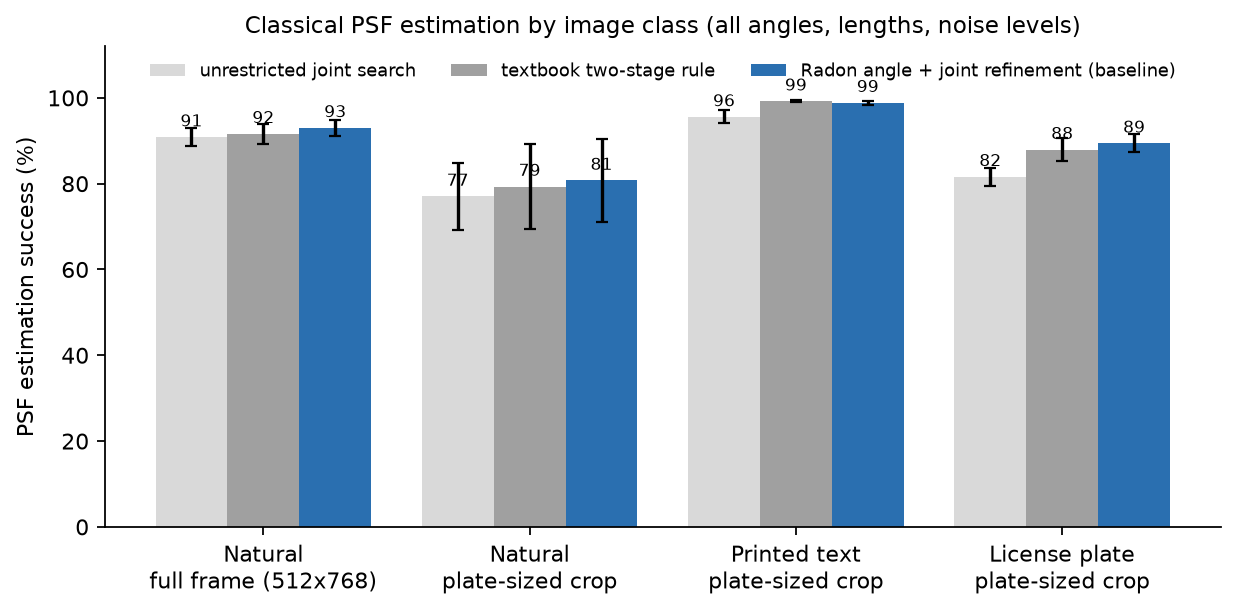
\includegraphics[width=0.66\textwidth]{02_success_by_class.png}
\caption{Estimation success on the test split (error bars: 95\% CI over source images). Three
angle strategies on identical trials; the baseline is the Radon-variance angle with a $\pm3^\circ$
joint refinement.}
\label{fig:sweepclass}
\end{figure}

\begin{table}[h]
\centering\small
\resizebox{\textwidth}{!}{\begin{tabular}{lcccc}
\toprule
 & natural, full frame & natural, crop & printed text, crop & plate, crop \\
\midrule
baseline (Radon angle + refinement) & \textbf{93.0} & \textbf{80.7} & 98.9 & \textbf{89.4} \\
textbook two-stage rule & 91.6 & 79.3 & \textbf{99.2} & 87.9 \\
unrestricted joint search & 90.9 & 77.0 & 95.6 & 81.6 \\
\midrule
baseline, $\sigma = 0.04$ & 80.3 & 60.6 & 96.2 & 75.6 \\
baseline, $L = 5$\,px & 71.3 & 56.1 & 94.9 & 58.1 \\
\midrule
PSNR blurred $\rightarrow$ restored (estimated PSF) & 24.6 $\rightarrow$ 25.3 & 23.2 $\rightarrow$ 23.5 & 15.6 $\rightarrow$ 17.7 & 20.3 $\rightarrow$ 22.7 \\
\quad restored with the true PSF (ceiling) & 26.0 & 24.7 & 17.8 & 23.6 \\
\quad restorations worse than the input & 6.3\% & 14.8\% & 0.7\% & 7.1\% \\
\bottomrule
\end{tabular}}
\caption{Success rate (\%) on the test split and restoration quality (RL with discrepancy stopping).}
\label{tab:sweep}
\end{table}

\begin{figure}[h]
\centering
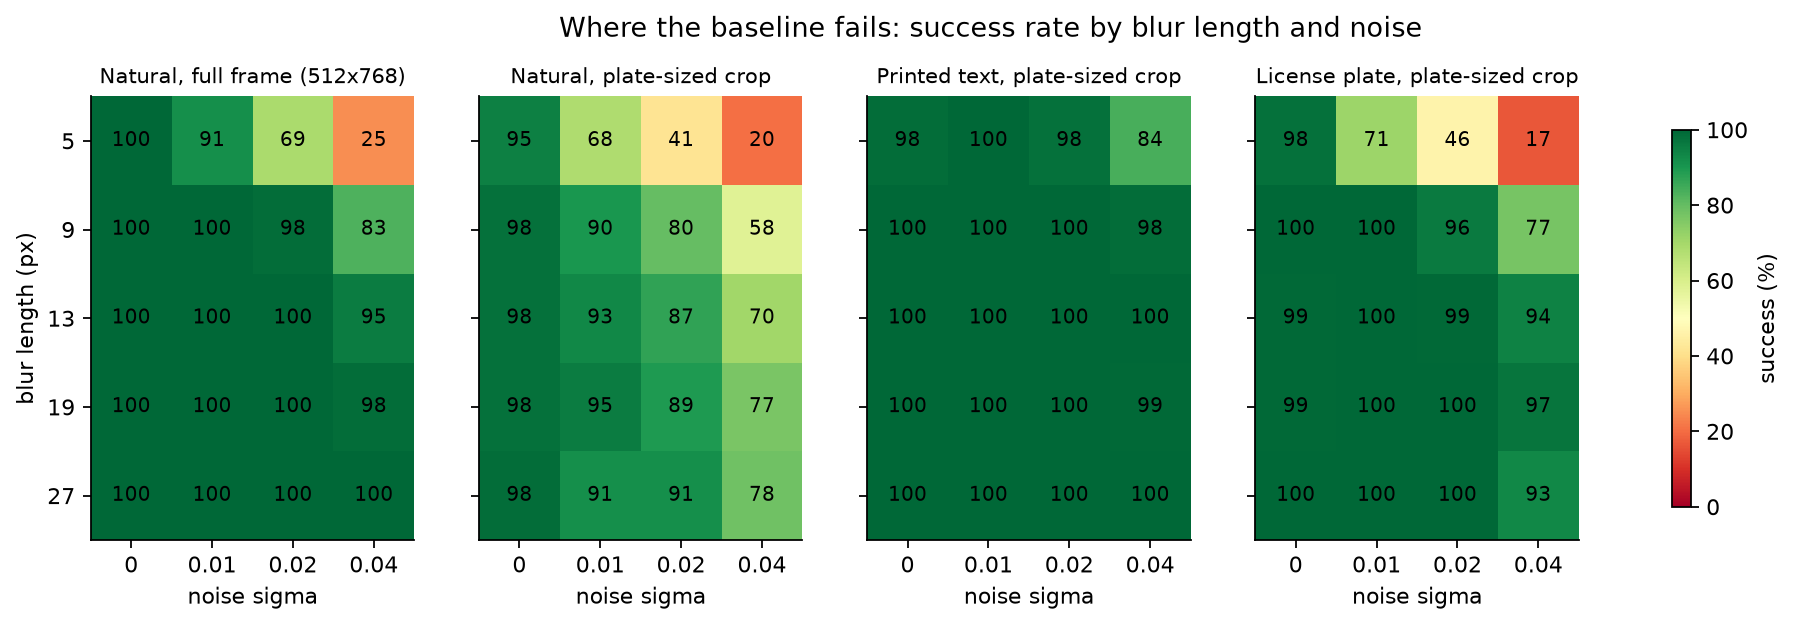
\includegraphics[width=\textwidth]{02_heatmap_length_noise.png}
\caption{Baseline success by blur length and noise level. The failure pocket is short blur under
noise, and it is much larger in a plate-sized window than at full frame.}
\label{fig:heat}
\end{figure}

\paragraph{Findings.} (i) The estimator is \emph{not} weaker on text content: printed text in a
plate-sized window is the easiest class (98.9\%), easier than natural texture in the same window
(80.7\%). Text is high-contrast and broadband, which is exactly what produces deep, regular sinc
nulls. (ii) What hurts is region size: the same Kodak images drop from 93.0\% at full frame to
80.7\% in the plate-sized window, because fewer samples carry the null pattern and the windowing
smears it. (iii) Within a window, the failures concentrate on short blurs under noise
(Fig.~\ref{fig:heat}): at $L=5$ the first null sits at $0.4$ of Nyquist, where noise dominates; at
$L\ge 13$ plates are above 94\% even at the highest noise level. (iv) Plates lie between text and
natural crops: the plate itself is high-contrast, but the window also holds bumper, grille and
background. (v) A wrong estimate is costly: in 7--15\% of the window trials the restoration with the
estimated PSF is worse than the blurred input, which is what the gate is for.

\paragraph{Angle strategy.} The Radon-variance angle is the more robust cue: the unrestricted joint
search, which phase~0 had favoured, has a 3--4$\times$ larger mean angle error (e.g.\ $7.1^\circ$ vs.\
$1.7^\circ$ on plates) because isolated deep dips in a wrong direction win the global minimum. The
$\pm3^\circ$ refinement around the Radon angle adds 1--2 points over the pure two-stage rule.
